\documentclass[12pt]{article}

\usepackage[T3]{fontenc}
\usepackage[utf8]{inputenc}
\usepackage[russian]{babel}

\usepackage{mhchem}
\usepackage{amssymb, amsmath}

\usepackage{tikz}
\usetikzlibrary{shapes.geometric, arrows, positioning, decorations.markings}
\usetikzlibrary{fit}
\usepackage{microtype}
\usepackage{framed}
\usetikzlibrary{decorations.pathmorphing,calc,backgrounds}

\usepackage{animate}

\usepackage{fixltx2e}
\usepackage{hyperref}

%\usetheme{Berkeley}
%\usetheme{Madrid} -- неплохо
%\usetheme{CambridgeUS}
%\usetheme{Singapore}
\usetheme{Warsaw}

\pdfmapfile{+sansmathaccent.map}

\title{Исследование бифуркаций в трехатомных гидридах методом классических траекторий}

\author{\small 
Финенко Артем \\[1ex] 
Научный руководитель: Петров С.В.}

\institute[MSU] % (optional, but mostly needed)
{
  МГУ им. М.В.Ломоносова \\
  Химический факультет
}

\date{23/12/2016}

\pgfdeclareimage[height=0.5cm]{university-logo}{../pictures/logo.jpg}
\logo{\pgfuseimage{university-logo}}

\newcommand\Fontvi{\fontsize{6}{7.2}\selectfont}

\beamertemplatenavigationsymbolsempty

\setbeamerfont{page number in head/foot}{size=\large}
\setbeamertemplate{footline}[frame number]
\setbeamertemplate{frametitle}[default][center]

% change font
\usefonttheme[onlymath]{serif}

% custom block environment
\newenvironment<>{varblock}[2][.9\textwidth]{%
  \setlength{\textwidth}{#1}
  \begin{actionenv}#3%
    \def\insertblocktitle{#2}%
    \par%
    \usebeamertemplate{block begin}}
  {\par%
    \usebeamertemplate{block end}%
  \end{actionenv}}

\tikzstyle{lagrange} = [rectangle, rounded corners, minimum width = 3cm, minimum height = 1cm, text centered, text width = 5cm, draw = black, fill=DarkOrchid!40]

\tikzstyle{equations} = [rectangle, rounded corners, text centered, draw = black, fill=green!30]

\tikzstyle{hamilton} = [rectangle, rounded corners, minimum width = 3cm, minimum height = 1cm, text centered, text width = 5 cm, draw = black, fill = Goldenrod!50]

\tikzstyle{result} = [rectangle, rounded corners, text centered, draw = black, fill = blue!30]

\tikzstyle{arrow} = [thick, ->, >=stealth]

\tikzstyle{vecArrow} = [thick, decoration={markings,mark=at position
   1 with {\arrow[semithick]{open triangle 60}}},
   double distance=1.4pt, shorten >= 5.5pt,
   preaction = {decorate},
   postaction = {draw,line width=1.4pt, white,shorten >= 4.5pt}]

\usepackage{caption}
\usepackage{subcaption}

\begin{document}

\begin{titlepage}
\centering
\textbf{\large Московский государственный университет имени М.В.\,Ломоносова\\
\vspace*{0.1cm} Химический факультет\\
\vspace*{0.1cm}
\noindent\makebox[\linewidth]{\rule{\paperwidth}{0.4pt}}
\vspace*{0.1cm}
 Кафедра физической химии\\
\vspace*{0.1cm} Лаборатория строения и квантовой механики молекул \\}
\vspace*{2cm}

\begin{center}

\includegraphics[width=0.3\textwidth]{pictures/logo.jpg}
\end{center}

\vspace*{2cm}
\Large \textbf{Расчет константы равновесия слабосвязанного комплекса $Ar-CO_2$}
\vspace*{2cm}

\begin{flushright}
\large Курсовая работа студента 411 группы\\
Финенко А.А.\\
\vspace{1cm}
Научные руководители:\\
к.ф.-м.н., с.н.с. Петров С.В. \\
м.н.с. Локштанов С.Е. \\
д. ф.-м.н., в.н.с. Вигасин А.А.
\end{flushright}
\vfill
\large\textbf{Москва\\ 2017}
\end{titlepage}



\tableofcontents
\newpage

\section{Схема получения полного колебательно-вращательного гамильтониана.}

Рассмотрим систему $n$ материальных точек. Обозначим их массы через $m_i$, их радиус-векторы в системе отсчета, cвязанной с  центром масс (такую систему в дальнейшем будем называть лабораторной), через $\mf{r}_i \, (i = 1, \dots n)$, в подвижной системе координат (также называемой молекулярной системой отсчета) -- через $\mf{R}_i \, (i = 1, \dots n)$. После отделения энергии центра масс кинетическая энергия в лагранжевой форме имеет следующий вид:
\vverh
\begin{gather}
	T_\mL = \frac{1}{2} \sum_{i=1}^{n} m_i \dot{\mf{r}}^2 \notag
\end{gather}

Переход от лабораторной системы отсчета к подвижной системе может быть осуществлен при помощи углов Эйлера $\varphi$, $\theta$ и $\psi$. Ортогональная матрица $\bbS$, связывающая координаты векторов в лабораторной и молекулярной системах отсчета является произведением матриц поворота:
\vverh
\begin{gather}
	\bbS = \bbS_\psi \, \bbS_\theta \, \bbS_\varphi =  
	\begin{bmatrix}
		\cos \psi & \sin \psi & 0 \\
		- \sin \psi & \cos \psi & 0 \\
		0 & 0  & 1
	\end{bmatrix}
	\begin{bmatrix}
		1 & 0 & 0 \\
		0 & \cos \theta & \sin \theta \\
		0 & - \sin \theta & \cos \theta 
	\end{bmatrix}
	\begin{bmatrix}
		\cos \varphi & \sin \varphi & 0 \\
		- \sin \varphi & \cos \varphi & 0 \\
		0 & 0 & 1
	\end{bmatrix} \notag \\
	\mf{a}_{\text{МСК}} = \bbS \, \mf{a}_{\text{ЛСК}} \quad \implies \quad \mf{R}_i = \bbS \mf{r}_i \notag
\end{gather}

В подвижной системе отсчета кинетическая энергия в лагранжевой форме имеет следующий вид:
\vverh
\begin{gather}
	T = \frac{1}{2} \sum_{i = 1}^{n} m_i \dot{\mf{R}}_i^2 + \mf{\Omega}^\top \sum_{i=1}^{n} m_i \left[ \mf{R}_i \times \dot{\mf{R}}_i \right] + \mf{\Omega}^{\top} \bbI \, \mf{\Omega} \notag
\end{gather}

Пусть исследуемая система содержит $s$ внутренних степеней свободы, тогда $\mf{R}_i = \mf{R}_i \lb \mf{q} \rb, \, \mf{q} = \lb q_1, \dots q_s \rb$. Подставляя выражение для радиус-векторов $\mf{R}_i$ через внутренние координаты, приходим к следующей форме кинетической энергии:
\vverh
\begin{gather}
	T_\mL = \frac{1}{2} \dot{\mf{q}}^\top \bba \dot{\mf{q}} + \mf{\Omega}^\top \bbA \, \dot{\mf{q}} + \frac{1}{2} \mf{\Omega}^\top \bbI \, \mf{\Omega}, \notag
\end{gather}

где $\bba_{jk} = \displaystyle \sum_{i=1}^{n} m_i \displaystyle \frac{\partial \mf{R}_i}{\partial q_j} \frac{\partial \mf{R}_i}{\partial q_k}$ -- матрица относительной кинетической энергии; \\ 
$\bbA_{jk} = \displaystyle \sum_{i=1}^{n} m_i \left[ \mf{R}_i \times \displaystyle \frac{\partial \mf{R}_i}{\partial q_k} \right]_\alpha$ (здесь $\alpha = x, y, z$ соответствуют $j = 1, 2, 3$) -- кориолисова матрица; $\bbI$ -- матрица тензора инерции. \par
Перепишем выражение для кинетической энергии в матричном виде, где матрица $\bbB$ представляет собой блочную матрицу:
\vverh
\begin{gather}
	T_\mL = \frac{1}{2}
	\begin{bmatrix}
		\mf{\Omega}^\top & \hspace*{-2mm} \dot{\mf{q}}^\top
	\end{bmatrix}
	\bbB
	\begin{bmatrix}
		\mf{\Omega} \\ 
		\dot{\mf{q}}
	\end{bmatrix},
	\quad \quad
	\bbB = 
	\begin{bmatrix}
		\bbI & \bbA \\
		\bbA^\top & \bba
	\end{bmatrix}
	\notag
\end{gather}

Запишем гамильтоновы переменные $\mf{p}$ и $\mf{J}$ как производные кинетической энергии в лагранжевом представлении. Заметим, что блочный вектор гамилтоновых переменных связан с блочным вектором лагранжевых переменных матрицей $\bbB$.
\vverh
\begin{gather}
	\begin{aligned}
		\mf{J} &= \frac{\partial T_\mL}{\partial \mf{\Omega}} = \bbI \, \mf{\Omega} + \bbA \, \dot{\mf{q}} \\
		\mf{p} &= \frac{\partial T_\mL}{\partial \dot{\mf{q}}} = \bbA^\top \mf{\Omega} + \bba \dot{\mf{q}}
	\end{aligned}
	\quad \implies \quad
	\begin{bmatrix}
		\mf{J} \\
		\mf{p}
	\end{bmatrix} = 
	\bbB
	\begin{bmatrix}
		\mf{\Omega} \\
		\dot{\mf{q}}
	\end{bmatrix} \notag
\end{gather}

Обращение блочной матрицы $\bbB$ легче всего осуществить воспользовавшись формулами Фробениуса. Обозначим $\bbG = \bbB^{-1} = \begin{bmatrix} \bbG_{11} & \bbG_{12} \\ \bbG_{21} & \bbG_{22} \end{bmatrix}$:
\vverh
\begin{gather}
	\begin{aligned}
		\bbG_{11} &= \lb \bbI - \bbA \bba^{-1} \bbA^\top \rb^{-1} \\
		\bbG_{12} &= - \bbI^{-1} \bbA \bbG_{22} = - \bbG_{11} \bbA \bba^{-1} \\
		\bbG_{21} &= - \bba^{-1} \bbA^\top \bbG_{11} = \bbG_{22} \bbA^\top \bbI^{-1} \\
		\bbG_{22} &= \lb \bba - \bbA^\top \bbI^{-1} \bbA \rb^{-1}
	\end{aligned} \notag
\end{gather}

Кинетическую энергию в гамильтоновом представлении получаем в результате стандартной процедуры:
\vverh
\begin{gather}
	T_\mH = 
	\begin{bmatrix}
		\mf{\Omega}^\top & \hspace*{-2mm} \dot{\mf{q}}
	\end{bmatrix}
	\begin{bmatrix}
		\mf{J} \\
		\mf{p}
	\end{bmatrix}
	- T_\mL = \frac{1}{2} 
	\begin{bmatrix}
		\mf{J} & \mf{p}
	\end{bmatrix}
	\bbG
	\begin{bmatrix}
		\mf{J} \\
		\mf{p}
	\end{bmatrix} = 
	\frac{1}{2} \mf{J}^\top \bbG_{11} \mf{J} + \frac{1}{2} \mf{p}^\top \bbG_{22} \mf{p} + \mf{J} \, \bbG_{12} \mf{p} \notag
\end{gather}




\section{Колебательно-вращательный гамильтониан системы $Ar-CO_2$}

Введем молекулярную систему отсчета: направим ось $OZ$ вдоль линии $C-Ar$, ось $OX$ через центр масс перпендикулярно ей в плоскости системы, ось $OY$ перпендикулярно плоскости системы. Обозначим массы атомом: кислорода -- $m_1$, аргона -- $m_2$, углерода -- $m_3$; обозначим $l$ расстояние $O-O$ в молекуле $CO_2$. Обозначим расстояние от атома $C$ до атома $Ar$ через $R$, угол между вектором $C-Ar$ и $CO_2$ -- через $\theta$. Пара переменных $R, \theta$ образуют систему внутренних координат (вектор $\mf{q}$ при формировании матриц, определяющих кинетическую форму в лагранжевом и гамильтоновых представлениях, используется в форме $\begin{bmatrix} R & \theta \end{bmatrix}$). Внутримолекулярные колебания $CO_2$ происходят существенно быстрее молекулярных движений рассматриваемой системы $Ar-CO_2$ и в среднем не взаимодействуют с ними. Поэтому будем считать молекулу $CO_2$ жесткой в рамках дальнейшего рассмотрения.  
\begin{figure}[h]
\centering
\begin{tikzpicture}
	[oxygen/.style={ball color = red, circle, text = white}, 
	carbon/.style={ball color = black!30, circle, text = white},
	argon/.style={ball color = blue, circle, text = white}]
	\node (z1) at (4.5, 3) {OZ};
	\node (z2) at (-1.5, -1) {}
		edge [->, thick] (z1);

	\node (x1) at (-1, 3.5) {OX};
	\node (x2) at (3.5, -1) {}
		edge [->, thick] (x1); 

	\node (carbon) [carbon] {C};
	\node (oxygen1) [oxygen, below right of = carbon] {O}
		edge [double, thick] (carbon);
	\node (oxygen2) [oxygen, above left of = carbon] {O}
		edge [double, thick] (carbon);
	\node[argon] (argon) at (3, 2) {Ar};

	\begin{scope}[on background layer]
	\node [fill=yellow!30,fit=(z1) (z2) (x1) (x2) (carbon) (oxygen1) (oxygen2)] {};
\end{scope}
\end{tikzpicture}
\caption{Молекулярная система отсчета для системы $Ar-CO_2$.}
\end{figure}

Введем следующие обозначения:
\vverh
\begin{gather}
	\mu_1 = \frac{m_1}{2}, \quad 
	\mu_2 = \frac{m_2 \lb 2 m_1 + m_3 \rb}{2 m_1 + m_2 + m_3} \notag
\end{gather}

Матрицы $\bba$, $\bbA$, $\bbI$, определяющие вид кинетической энергии в лагранжевой форме: 
\vverh
\begin{gather}
	\bba =
	\begin{bmatrix}
		\mu_2 & 0 \\
		0 & \mu_1 l^2
	\end{bmatrix} \quad 
	\bbA = 
	\begin{bmatrix}
		0 & 0 \\
		0 & \mu_1 l^2 \\
		0 & 0 
	\end{bmatrix} \quad
	\bbI = 
	\begin{bmatrix}
		\mu_1 l^2 \cos^2 \theta + \mu_2 R^2 & 0 & -\mu_1 l^2 \sin \theta \cos \theta \\
		0 & \mu_1 l^2 + \mu_2 R^2 & 0 \\
		- \mu_1 l^2 \sin \theta \cos \theta & 0 & \mu_1 l^2 \sin^2 \theta
	\end{bmatrix} \notag
\end{gather}

Используя формулы Фробениуса, получаем матрицы $\bbG_{11}$, $\bbG_{12}$, $\bbG_{22}$, определяющие кинетическую энергию в гамильтоновой форме:
\vverh
\begin{gather}
	\bbG_{11} =
	\begin{bmatrix}
		\dfrac{1}{\mu_2 R^2} & 0 & \dfrac{\ctg \theta}{\mu_2 R^2} \\
		0 & \dfrac{1}{\mu_2 R^2} & 0 \\
		\dfrac{\ctg \theta}{\mu_2 R^2} & 0 & \dfrac{\ctg^2 \theta}{\mu_2 R^2} + \dfrac{1}{\mu_1 l^2 \sin^2 \theta}
	\end{bmatrix} \quad
	\bbG_{12} =
	\begin{bmatrix}
		0 & 0 \\
		0 & - \dfrac{1}{\mu_2 R^2} \\
		0 & 0
	\end{bmatrix} \quad 
	\bbG_{22} = 
	\begin{bmatrix}
		\dfrac{1}{\mu_2} & 0 \\
		0 & \dfrac{1}{\mu_2 R^2} + \dfrac{1}{\mu_1 l^2}
	\end{bmatrix} \notag
\end{gather}

Получаем гамильтониан системы $Ar-CO_2$ в заданной молекулярной системе координат:
\begin{gather}
\mH = \frac{1}{2 \mu_2} p_R^2 + \lb \frac{1}{2 \mu_2 R^2} + \frac{1}{2 \mu_1 l^2} \rb p_\theta^2 - \frac{1}{\mu_2 R^2} p_\theta J_y + \frac{1}{2 \mu_2 R^2} J_y^2 + \frac{1}{2 \mu_2 R^2} J_x^2 + \frac{1}{2 \sin^2 \theta} \lb \frac{\cos^2 \theta}{\mu_2 R^2} + \frac{1}{\mu_1 l^2} \rb J_z^2 + \notag \\
+ \frac{\ctg \theta}{\mu_2 R^2} J_x J_z + U(R, \theta) \notag
\end{gather}





\section{Поверхность потенциальной энергии межмолекулярного взаимодействия}

\begin{figure}[!h]
	\hspace*{-1.2cm}
	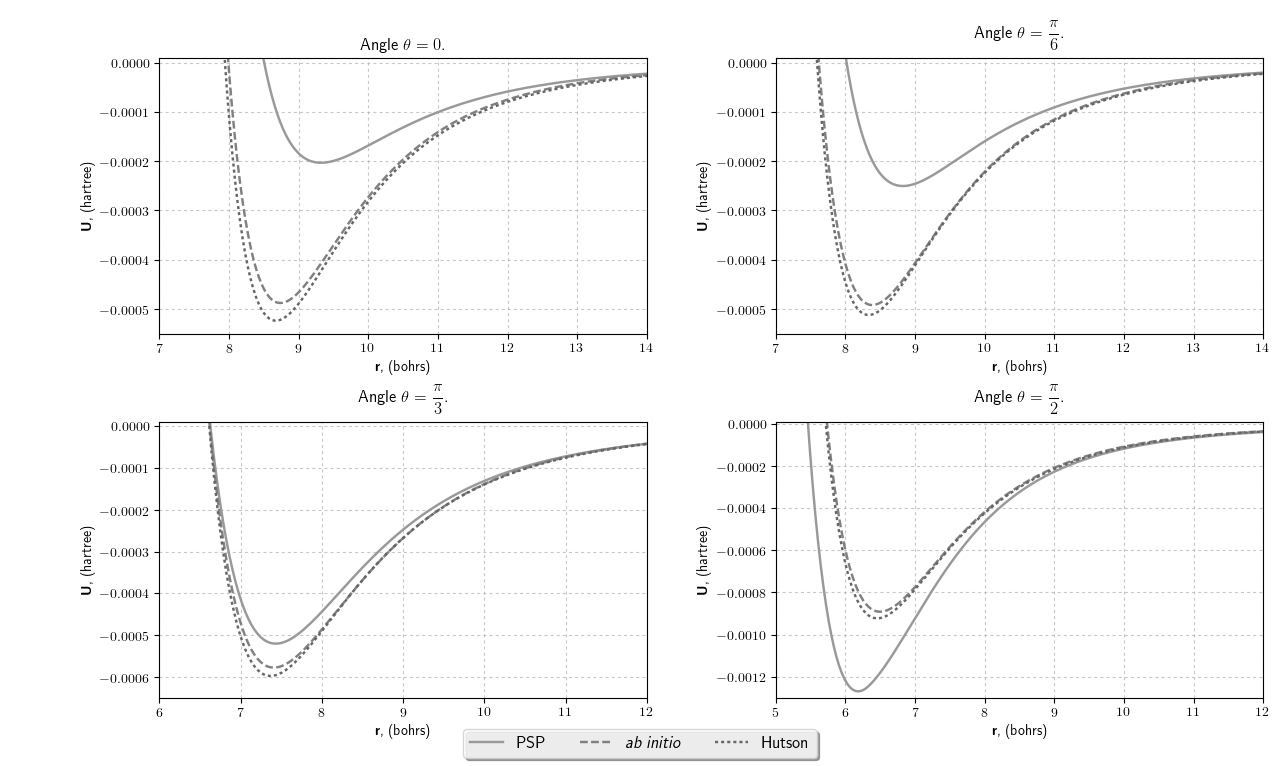
\includegraphics[width=1.1\textwidth]{pictures/potential_well.png}
	\caption{Сечения поверхностей потенциальной энергии при разных углах $\theta$ в области потенциальной ямы.}
\end{figure}

\begin{figure}[!h]
	\hspace*{-1.2cm}
	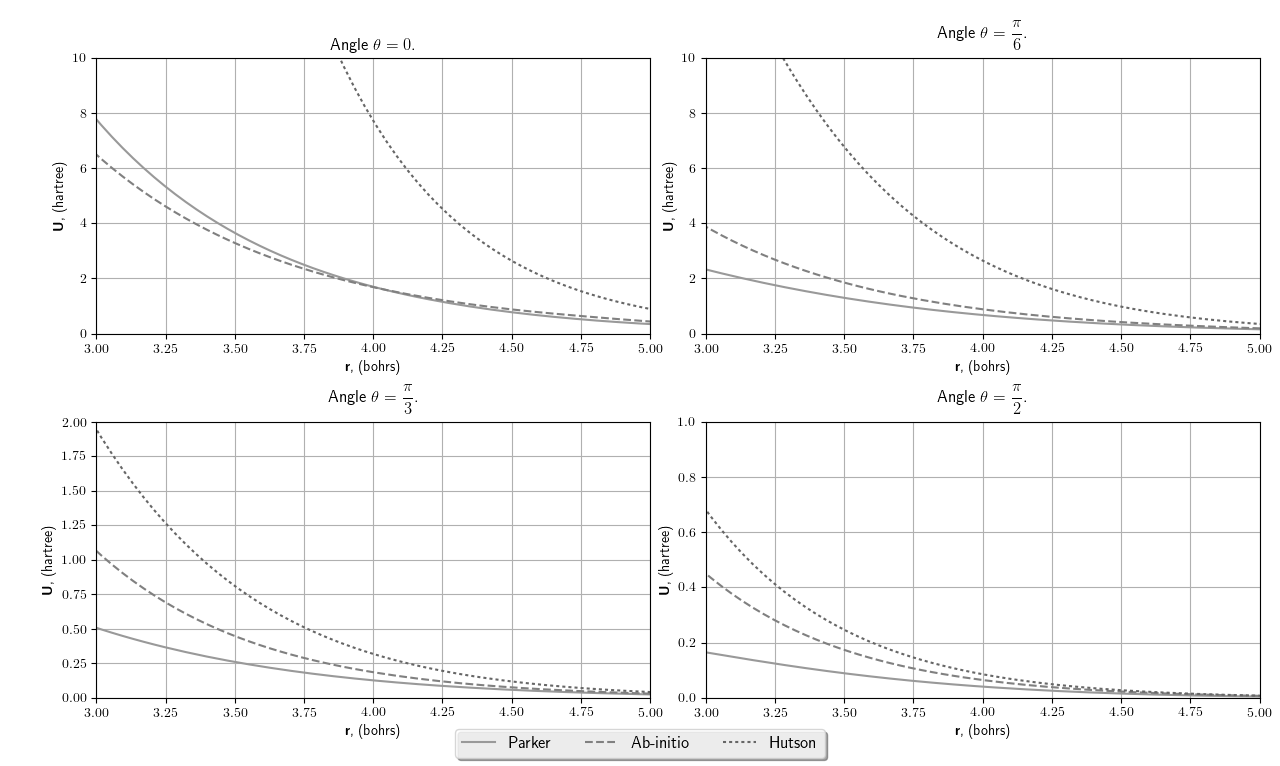
\includegraphics[width=1.1\textwidth]{pictures/potential_wall.png}
	\caption{Сечения поверхностей потенциальной энергии при разных углах $\theta$ в области потенциальной стены.}
\end{figure}

Первая поверхность потенциальной энергии (обозначаемая далее P.) для системы $Ar-CO_2$ была предложена в работе \cite{parker1976}. Потенциал P. имеет потенциальную яму, которая резко выражена для Т-образной геометрии. Потенциал представлен в виде следующего разложения по полиномам Лежандра:
\vverh
\begin{gather}
	U(r, \theta) = \sum_{n = 0, 2 \dots} v_n(r) P_n \lb \cos \theta \rb, \notag
\end{gather}
в котором появляются только четные $n$ из-за $D_{\infty h}$ симметрии молекулы $CO_2$. Функции $v_n(r)$ при малых расстояниях представляют собой экспоненциальные функции (описывают резкое возрастание потенциальной поверхности), при больших расстояниях -- полиномиальные функции (описывающие Ван-дер-Ваальсово притяжение). 
\vverh
\begin{gather}
	v_n^{HF} = A_{n1} \exp \lb A_{n2} r + A_{n3} r^2 \rb, \notag \quad \quad 
	v_n^{COR} = \left\{
	\begin{aligned}
		- B_{n1}^{\, \prime} \exp \lb B_{n2} + B_{n3} r^2 \rb, \quad r \leqslant r_n \\
		-C_6(n) r^{-6} - C_8(n) r^{-8}, \quad r \geqslant r_n
	\end{aligned} \right. \notag \\
	v_n(r) = v_n^{HF} + v_n^{COR} \notag 
\end{gather}

Вторая поверхность потенциальной энергии была взята из работы \cite{hutson1996}. Т.к. эта работа была выполнена практически спустя 20 лет после первой, экспериментальные данные, на которые опирались авторы при построении потенциальной поверхности, в значительной степени пополнились. Построенная ППЭ опирается на спектроскопические данные высокого разрешения и на температурную зависимость вириального коэффициента. Аналитическое представление потенциала также было выполнено путем разложения в ряд по полиномам Лежандра.  

Наконец, третья поверхность была построена Калугиной Ю. путем проведения \textit{ab-initio} расчета (CC) ... 
УЗНАТЬ ЧТО НАПИСАТЬ ПРО ПОТЕНЦИАЛ ЮЛИ


Профили потенциальной энергии при $T$-образной геометрии комплекса (соответствуют $\theta = \ddfrac{\pi}{2}$) показывают, что потенциал P. имеет существенно большую яму чем другие два потенциала, которые при данной геометрии отличаются достаточно не существенно. При уменьшении угла $\theta$ видно, что разница между потенциалами H. и \textit{ab-initio} также остается достаточно несущественной, в то время как потенциальная яма P. резко изменяет свою величину с уменьшением угла $\theta$. Однако интегральная величина потенциальной ямы (усредненная по угловой координате) оказывается близка для потенциалов H. и P. \cite{hutson1996}. \par
В области потенциальной стены соотношение между потенциалами изменяется. Самым быстрым является потенциал H., потенциалы P. и \textit{ab-initio} оказываются близки при линейной геометрии, однако при других геометриях устанавливается следующий порядок между потенциалами (по возрастанию значений): P., \textit{ab-initio}, H.



\section{Расчет второго вириального коэффициента и квантовых поправок}




\newpage

\section{Константа равновесия системы $Ar-CO_2$}

\subsection{Константа равновесия в каноническом ансамбле \cite{keszei, landau2}}

Канонический ансамбль представляет собой модель термодинамической системы, погруженной в тепловой резервуар постоянной температуры. В представленной системе резервуар играет роль термостата, поддерживая температуру исследуемой системы постоянной независимо от направления теплового потока. Канонический ансамбль (также называемый $NVT$-ансамблем) представляет собой систему из $N$ частиц, находящихся в фиксированном объеме $V$ при фиксированной температуре $T$. Отметим, что энергия $NVT$-ансамбля может принимать любые значения, согласующиеся с заданными условиями. Рассматривая совокупность резервуара и погруженной в него исследуемой системы как микроканонический ансамбль, получают каноническое распределение (распределение Гиббса) -- вероятность нахождения системы в состоянии с энергией $E_n$:
\vverh
\begin{gather}
	\omega_n = A \times \exp \lb - \frac{E_n}{kT} \rb \quad \Leftrightarrow \quad \rho \lb p, q \rb = A \times \exp \lb - \frac{E \lb p, q \rb}{kT} \rb \notag
\end{gather}
Энтропия может быть выражена как среднее значение функции распределения:
\vverh
\begin{gather}
	S = - \langle \ln \omega_n \rangle \notag \\
	S = - \ln A + \frac{1}{T} \langle E_n \rangle = - \ln A + \frac{\overline{E}}{kT} \notag \\
	\ln A = \frac{\overline{E} - TS}{kT} = \frac{F}{kT} \notag 
\end{gather}
Средняя энергия $\overline{E}$ есть как раз то, что понимается в термодинамике под энергией $U$, таким образом получаем следующие выражение для функции распределения Гиббса через свободную энергию Гельмгольца (в квантовой и классической статистиках, соответственно):
\vverh
\begin{gather}
	\omega_n = \exp \lb - \frac{F - E_n}{kT} \rb \quad \Leftrightarrow \quad \rho(p, q) = \frac{1}{\lb 2 \pi \hbar \rb^{s}} \exp \lb \frac{F - E(p, q)}{kT} \rb \notag
\end{gather}

Условие нормировки для распределения $\omega_n$:
\vverh
\begin{gather}
	\sum_n \omega_n = \exp \lb \frac{F}{kT} \rb \sum_n \exp \lb - \frac{E_n}{kT} \rb = 1 \notag \\
	F = - kT \ln \sum_n \exp \lb - \frac{E_n}{kT} \rb = - kT \ln Z \notag
\end{gather}

При записи аналогичной формулы в классической термодинамике следует учесть, что если, например, переменить местами два одинаковых атома, то после такой перестановки микросостояние тела будет изображаться другой фазовой точкой, получающейся из первоначальной заменой и импульсов одного атома координатами и импульсами другого. С другой стороны, ввиду одинаковости переставляемых атомов, оба состояния тела физически тождественны. Таким образом, одному и тому же физическому микросостоянию тела в фазовом пространстве соответствует целый ряд точек. При интегрировании распределения каждое состояние должно учитываться лишь однократно (статистический интеграл можно рассмотреть как предел квантовой статистической суммы, суммирование в которой производится по всем различным квантовым состояниям), то есть, интегрирование производится лишь по тем областям фазового пространства, которые соответсвуют физически различным состояниям тела (штрих над интегралом будет подчеркивать эту особенность классической статистической суммы).
\vverh
\begin{gather}
	F = -k T \ln \int^{\prime} \exp \lb - \frac{E(p, q)}{kT} \rb d \Gamma, \quad d \Gamma = \frac{dp \, dq}{\lb 2 \pi \hbar \rb^s} \notag
\end{gather}

Запишем свободную энергию Гельмгольца, используя молекулярную статистическую сумму $q$. (Слагаемое $F(0)$ призвано подправить значение в правой части равенства, принимая во внимание свободу выбора начала отсчета для молекулярной суммы по состояниям.)  
\vverh
\begin{gather}
	F = - k T \ln Q = F(0) - kT \ln \frac{q^N}{N!} = F(0) - NkT \ln q + NkT \lb \ln N - 1 \rb \notag 
\end{gather}

Полагая $N = N_A$, приходим к мольному значению свободной энергии Гельмгольца:
\vverh
\begin{gather}
	F_m = F_m(0) - RT \ln \frac{q}{N_A} - RT \notag
\end{gather}

В приближении идеального газа имеем $G_m = F_m + p V_m = F_m + RT$. Заметим, что $F_m(0) = U_m(0)$. Под $q^{\barcirc} = q_{NVT}^{\barcirc}$ понимается значение суммы по состояниям, вычисленное при $N = N_A$, фиксированной температуре $T$ и при фиксированном объеме $V = \frac{RT}{p^{\barcirc}}$.
\vverh
\begin{gather} 
	G_m = F_m(0) - RT \ln \frac{q}{N_A} \notag \\
	G^{\barcirc} = U_m(0) - RT \ln \frac{q^{\barcirc}}{N_A} \notag \\
	\Delta_r G^{\barcirc} = \Delta_r U_m(0) - RT \ln \prod_{i} \lb \frac{q_i^{\barcirc}}{N_A} \rb ^{\nu_i} \notag
\end{gather}

Используя равенство $\Delta_r G^{\barcirc} = - RT \ln K$, получаем выражение для термодинамической константы равновесия:
\vverh
\begin{gather}
	K = \prod_{i = 1}^{r} \lb \frac{q_i^{\barcirc}}{N_A} \rb^{\nu_i} \exp \lb - \frac{\Delta_r U_m (0)}{RT} \rb \notag
\end{gather}

Термодинамическая и газовая константы равновесия связаны между собой следующим соотношением: 
\vverh
\begin{gather}
	K_p =  K \times \lb p^{\barcirc} \rb^{\sum_i \nu_i} \notag 
\end{gather}

Получим выражение для газовой константы равновесия $K_p$ слабосвязанного комплекса $Ar-CO_2$. В условиях совпадающего начала отсчета молекулярных сумм по состояниям для всех участников реакции, получаем следующее выражение:
\vverh
\begin{gather}
	K_p = \frac{N_A}{p^{\barcirc}} \frac{q_{Ar-CO_2}^{\barcirc}}{q_{Ar}^{\barcirc} q_{CO_2}^{\barcirc}} \label{eqconst}
\end{gather}

\subsection{Статистическая сумма связанного димера} 

Связанным димером называют пару мономеров, энергия которых меньше чем у пары мономеров на бесконечно большом расстоянии друг от друга. Следовательно, классическая сумма по состояниям связанного димера представляет собой следующий фазовый интеграл
\vverh
\begin{gather}
	Q_{bound}^{pair} = \frac{1}{h^8} \int\limits_{H - \ddfrac{\strut P_{cm}^2}{\strut 2 M} < 0} \exp \lb - \frac{H}{k T} \rb d x_{cm} d y_{cm} d z_{cm} d P_{x} d P_{y} d P_{z} d q_i d p_i, \label{ci1}
\end{gather}

где $q_i$, $p_i$ -- набор внутримолекулярных координат и импуьсов, $H$ - гамильтониан, записанный в лабораторной системе координат, $\mathbf{R} = \lb x_{cm}, y_{cm}, z_{cm} \rb$, $\mathbf{P}_R = \lb P_x, P_y, P_z \rb$ -- векторы координат и импульсов центра масс, а $M$ -- его масса. \par
Отметим, что гамильтониан, фигурирующий в выражении \eqref{ci1}, связан с гамильтонианом в молекулярно-фиксированной системе отсчета соотношением
\vverh
\begin{gather}
	H = \mH + \frac{P_{cm}^2}{2 M} \notag
\end{gather}

Интегрирование по векторам центра масс $\mf{R}$, $\mf{P}_R$ в выражении \eqref{ci1} дает трансляционную статистическую сумму димера:
\vverh
\begin{gather}
	\lb Q_{bound}^{pair} \rb_{tr} = \lb \frac{2 \pi M k T}{h^2} \rb^{\frac{3}{2}} V \notag
\end{gather}

\subsection{Эйлеровы углы и сопряженные им импульсы}
Рассмотрим кинетическую энергию в лагранжевой форме
\vverh
\begin{gather}
	T_\mL = \frac{1}{2} \dot{\mf{q}}^\top \bba \, \dot{\mf{q}} + \mf{\Omega}^\top \bbA \dot{\mf{q}} + \frac{1}{2} \mf{\Omega}^\top \bbI \, \mf{\Omega} \notag
\end{gather}
Вектор угловой скорости $\mf{\Omega}$ связан с вектором эйлеровых скоростей $\dot{\mf{e}}$ при помощи матрицы $\bbV$ \cite{goldstein}:
\begin{gather}
\mathbf{\Omega} = \mathbb{V} \dot{\mathbf{e}} = 
\begin{bmatrix}
\sin \theta \sin \psi & \cos \varphi & 0 \\
\sin \theta \cos \psi & - \sin \psi & 0 \\
\cos \theta & 0 & 1
\end{bmatrix}
\begin{bmatrix}
\dot{\varphi} \\
\dot{\theta} \\
\dot{\psi}
\end{bmatrix} \notag 
\end{gather}

По определению построим вектор эйлеровых импульсов:
\vverh
\begin{gather}
	\mf{p}_e = \frac{\partial T_\mL}{\partial \dot{\mf{e}}} = \bbV^\top \bbA \dot{\mf{q}} + \bbV^\top \bbI \, \bbV \dot{\mf{e}} = \bbV^\top \bbA \dot{\mf{q}} + \bbV^\top \bbI \, \mf{\Omega} \notag
\end{gather}

Несложно показать, что вектор углового момента в подвижной системе отсчета равен
\vverh
\begin{gather}
	\mf{J} = \frac{\partial \mL}{\partial \mf{\Omega}} = \bbA \dot{\mf{q}} + \bbI \, \mf{\Omega} \notag
\end{gather}

Таким образом, получаем следующую связь между вектором эйлеровых импульсов и вектором углового момента:
\vverh
\begin{gather}
	\mf{J} = \lb \bbV^\top \rb^{-1} \mf{p}_e \notag
\end{gather}

Интегрирование в \eqref{ci1} в том числе ведется по эйлеровым углам и импульсам. В связи с этим рассмотрим следующий кратный интеграл и осуществим в нем замену переменных $p_\varphi, p_\theta, p_\psi \longrightarrow J_x, J_y, J_z$. (В этом подразделе $\theta$ -- один из эйлеровых углов, а не внутренняя система координата системы $Ar-CO_2$. Эта замена нам интересна по той причине, что в выражение гамильтониана входят именно компоненты углового момента, а не эйлеровы импульсы; так выражение получается намного более компактным.)
\vverh
\begin{gather}
	\int\limits_{0}^{2 \pi} d \varphi \int\limits_{0}^{\pi} d \theta \int\limits_{0}^{2 \pi} d \psi \int d p_\varphi \int d p_\theta \int d p_\psi = \int \, \left[ Jac \right] d J_x \int d J_y \int d J_z \notag
\end{gather}

Якобиан замены переменных равен
\vverh
\begin{gather}
	\left[ Jac \, \right] = \Bigg{|} \frac{\partial \mathbf{p}}{\partial \mathbf{J}} \Bigg{|} = \Bigg{|} \det \lb \bbV^\top \rb \Bigg{|} = \sin \theta \notag
\end{gather}

Если подынтегральное выражение не зависит от эйлеровых углов (как в случае со стастической суммой связанного димера), то интегральное выражение преобразуется к виду
\vverh
\begin{gather}
	\int\limits_{0}^{2 \pi} d \varphi \int\limits_{0}^{\pi} d \theta \int\limits_{0}^{2 \pi} d \psi \int d p_\varphi \int d p_\theta \int d p_\psi = 8 \pi^2 \int d J_x \int d J_y \int d J_z \notag 
\end{gather}

Однако, в случае системы $Ar-CO_2$ вращение на углы $\psi$ большие чем $\pi$ не приводит к новым состояниям системы (из-за симметричности молекулы $CO_2$), следовательно для рассматриваемой системы интегральное выражение имеет вид
\vverh
\begin{gather}
	\int\limits_{0}^{2 \pi} d \varphi \int\limits_{0}^{\pi} d \theta \int\limits_{0}^{\pi} d \psi \int d p_\varphi \int d p_\theta \int d p_\psi = 4 \pi^2 \int d J_x \int d J_y \int d J_z \notag 
\end{gather}

\subsection{Упрощенный вид суммы по состояниям связанного димера}

Заменяя эйлеровы импульсы на компоненты углового момента и интегрируя по переменным центра масс, сводим интеграл \eqref{ci1} к следующему:
\vverh
\begin{gather}
	Q_{bound}^{pair} = \lb Q_{bound}^{pair} \rb_{tr} \frac{4 \pi^2}{h^5} \int\limits_{\mH < 0} \exp \lb - \frac{\mH}{kT} \rb d R \, d \theta \, d p_R \, d p_\theta \, d J_x \, d J_y \, d J_z. \notag
\end{gather}

Рассмотрим гамильтониан системы $Ar-CO_2$ в молекулярно-фиксированной системе координат:
\begin{gather}
	\mH = \frac{1}{2 \mu_2} p_R^2 + \lb \frac{1}{2 \mu_2 R^2} + \frac{1}{2 \mu_1 l^2} \rb p_\theta^2 - \frac{1}{\mu_2 R^2} p_\theta J_y + \frac{1}{2 \mu_2 R^2} J_y^2 + \frac{1}{2 \mu_2 R^2} J_x^2 + \frac{1}{2 \sin^2 \theta} \lb \frac{\cos^2 \theta}{\mu_2 R^2} + \frac{1}{\mu_1 l^2} \rb J_z^2 + \notag \\
+ \frac{\ctg \theta}{\mu_2 R^2} J_x J_z + U(R, \theta) \notag
\end{gather}

Заметим, что форма гамильтониана $\mH$ позволяет представить его в виде положительно определенной квадратичной формы:
\begin{gather}
	\mH = \frac{p_R^2}{2 \mu_2} + \frac{p_\theta^2}{2 \mu_1 l^2} + \frac{1}{2 \mu_2 R^2} \lb p_\theta - J_y \rb^2 + \frac{1}{2 \mu_2 R^2} \lb J_x + J_z \ctg \theta \rb^2 + \frac{J_z^2}{2 \mu_1 l^2 \sin^2 \theta} + U(R, \theta) \notag
\end{gather}

Дальнейшие преобразования основаны на анализе фазового интеграла, представленном в работе \cite{vigasin2015}. Подготовим следующую линейную замену переменных $p_R, p_\theta, J_x, J_y, J_z \rightarrow x_1, x_2, x_3, x_4, x_5$ (причем $R, \theta$ считаем постоянными при осуществлении замены), упрощающую подэкспоненциальное выражение (впервые предложена в \cite{ozaki1985}):
\vverh
\begin{gather}
	\hspace*{-0.5cm}
	\everymath{\scriptstyle}
	\footnotesize
	\left\{
	\begin{aligned}
	x_1^2 &= \frac{p_R^2}{2 \mu_2 kT} \\
	x_2^2 &= \frac{p_\theta^2}{2 \mu_1 l^2 kT} \\
	x_3^2 &= \frac{ \lb p_\theta - J_y \rb^2}{2 \mu_2 R^2 k T} \\
	x_4^2 &= \frac{ \lb J_x + J_z \ctg \theta \rb^2}{2 \mu_2 R^2 k T} \\
	x_5^2 &= \frac{J_z^2}{2 \mu_1 l^2 \sin^2 \theta kT}
	\end{aligned}
	\right. \quad \implies \quad 
	\left\{
	\begin{aligned}
	dx_1 &= \frac{dp_R}{\sqrt{ 2 \mu_2 k T}} \\
	dx_2 &= \frac{dp_\theta}{\sqrt{2 \mu_1 l^2 k T}} \\
	dx_3 &= \frac{dp_\theta - dJ_y}{\sqrt{2 \mu_2 R^2 k T}} \\
	dx_4 &= \frac{dJ_x + \ctg \theta dJ_z}{ \sqrt{2 \mu_2 R^2 k T}} \\
	dx_5 &= \frac{dJ_z}{\sqrt{2 \mu_1 l^2 \sin^2 \theta k T}}
	\end{aligned}
	\right. \quad \implies \quad
	\left\{
	\begin{aligned}
		dp_R &= \sqrt{2 \mu_2 k T} dx_1 \\
		dp_\theta &= \sqrt{2 \mu_1 l^2 kT} dx_2 \\
		dJ_y &= \sqrt{2 \mu_1 l^2 kT} dx_2 - \sqrt{2 \mu_2 R^2 kT} dx_3 \\
		dJ_x &= \sqrt{2 \mu_2 R^2 kT} dx_4 - \sqrt{2 \mu_1 l^2 \cos^2 \theta kT} dx_5 \\
		dJ_z &= \sqrt{2 \mu_1 l^2 \sin^2 \theta kT} dx_5
	\end{aligned}
	\right.
	\notag
\end{gather}

Для упрощения выражений откинем на время трансляционную статистическую сумму димера и $4 \pi^2$. Основываясь на теореме Фубини, интеграл \eqref{ci1} может быть представлен в виде повторного интеграла, в котором сначала интегрирование ведется по переменным $p_R$, $p_\theta$, $J_x$, $J_y$, $J_z$, а затем  -- по переменным $R, \theta$. Таким образом, во внутреннем интеграле переменные $R, \theta$ являются постоянными, что позволяет осуществить приготовленную замену:
\vverh
\begin{gather}
	\frac{1}{h^5} \int_{H < 0} \exp \lb -\frac{\mH}{kT} \rb dR \, dp_R \, d \theta \, dp_\theta \, d J_x \, d J_y \, d J_z = \frac{1}{h^5} \iint dR \, d \theta \int \exp \lb -\frac{\mH}{kT} \rb d p_R \, d p_\theta \, d J_x \, d J_y \, d J_z = \notag \\
	= \frac{1}{h^5} \iint  \left[ Jac \, \right] \exp \lb -\frac{U}{kT} \rb d R \, d \theta \times \idotsint\limits_{x_1^2 + \dots + x_5^2 + \frac{U}{kT} < 0} \exp \lb - x_1^2 - \dots - x_5^2 \rb dx_1 \dots dx_5, \notag 
\end{gather}

\vlevo где якобиан замены переменных $\left[ Jac \, \right]$ равен следующему произведению радикалов: 
\begin{gather}
	\hspace*{-1.0cm}
	\left[ Jac \, \right] = \Bigg{|} \frac{\partial [p_R, p_\theta, J_x, J_y, J_z]}{\partial [x_1, x_2, x_3, x_4, x_5]} \Bigg{|} = \det  
	\begin{bmatrix}
		\sqrt{2 \mu_2 k T} & 0 & 0 & 0 & 0 \\
		0 & \sqrt{2 \mu_1 l^2 k T} & 0 & 0 & 0 \\
		0 & 0 & 0 & \sqrt{2 \mu_2 R^2 k T} & -\sqrt{2 \mu_1 l^2 \cos^2 \theta} \\
		0 & \sqrt{2 \mu_1 l^2 k T} & -\sqrt{2 \mu_2 R^2 k T} & 0 & 0 \\
		0 & 0 & 0 & 0 & \sqrt{2 \mu_1 l^2 \sin^2 \theta k T}
	\end{bmatrix} = \notag \\
	= \sqrt{2 \mu_2 k T} \sqrt{2 \mu_1 l^2 k T} \sqrt{2 \mu_2 R^2 kT} \sqrt{2 \mu_2 R^2 kT} \sqrt{2 \mu_1 l^2 \sin^2 \theta kT} = (2 \mu_2 kT)^\frac{3}{2} 2\mu_1 l^2 k T R^2 \sin \theta \notag
\end{gather}

Интеграл функции $\exp \lb - x_1^2  - x_2^2 - \dots - x_n^2 \rb$ по объему $n$-мерного шара с радиусом $R$ есть (доказательство этого соотношения приведено в приложении \eqref{appendix:multint})
\vverh
\begin{gather}
	\idotsint\limits_{x_1^2 + \dots + x_n^2 \leqslant R} \exp \lb -x_1^2 - x_2^2 - \dots - x_n^2 \rb d x_1 \dots d x_n = \pi^\frac{n}{2} \frac{\gamma \lb \frac{n}{2}, R^2 \rb}{\Gamma \lb \frac{n}{2} \rb}, \notag
\end{gather}
где $\gamma(a, b)$ -- неполная гамма-функция:
\vverh
\begin{gather}
	\gamma \lb a, b \rb = \int\limits_0^b \omega^{a - 1} \exp \lb - \omega \rb d \omega \notag
\end{gather}

Применяя общее соотношение для 5-мерного случая, получаем:
\vverh
\begin{gather}
	\idotsint\limits_{x_1^2 + \dots  + x_5^2 \leqslant -\frac{U}{k T}} \exp \lb - x_1^2 - \dots - x_5^2 \rb d x_1 \dots d x_5 = \pi^\frac{5}{2} \frac{\gamma \lb \frac{5}{2}, - \frac{U}{k T} \rb}{\Gamma \lb \frac{5}{2} \rb} \notag
\end{gather}

Итак, фазовый интеграл представлен в виде интеграла по переменным $R, \theta$ и интеграла по объему 5-мерного шара, радиус которого определяется значением потенциальной функции $U(R, \theta)$. Заметим, что радиус шара является ненулевым только при отрицательных значениях потенциальной функции $U(R, \theta)$, следовательно фазовый интеграл принимает ненулевые значения только в том случае, если переменные $R, \theta$ лежат в области $U < 0$.
\vverh
\begin{gather}
	\hspace*{-9cm} \frac{1}{h^5} \iint d R \, d \theta \int \exp \lb -\frac{\mH}{k T} \rb d p_R  \, dp_\theta \, dJ_x \, dJ_y \, dJ_z = \notag \\
	\hspace{5cm} =\lb \frac{2 \pi \mu_2 k T}{h^2} \rb^{\frac{3}{2}} \frac{2 \mu_1 l^2 \pi k T}{h^2} \iint\limits_{U < 0} \exp \lb -\frac{U}{k T} \rb \frac{\gamma \lb \frac{5}{2}, - \frac{U}{k T} \rb}{\Gamma \lb \frac{5}{2} \rb} R^2 \sin \theta dR \, d\theta \notag 
\end{gather}

Итак, выражение для статистической суммы связанного димера принимает вид:
\vverh
\begin{gather}
	Q_{bound}^{pair} = 4 \pi^2 \lb \frac{2 \pi M k T}{h^2} \rb^{\frac{3}{2}} V \lb \frac{2 \pi \mu_2 k T}{h^2} \rb^{\frac{3}{2}} \frac{2 \mu_1 l^2 \pi k T}{h^2} \iint\limits_{U < 0} \exp \lb -\frac{U}{k T} \rb \frac{\gamma \lb \frac{5}{2}, - \frac{U}{k T} \rb}{\Gamma \lb \frac{5}{2} \rb} R^2 \sin \theta dR \, d\theta \notag
\end{gather}
Заметим, что предынтегральные множители могут быть выражены через статистические суммы мономеров:
\vverh
\begin{gather}
	Q_{CO_2} = Q_{CO_2}^{tr} Q_{CO_2}^{rot} = \lb \frac{2 \pi m_{CO_2} k T}{h^2} \rb^{\frac{3}{2}} V \frac{4 \pi^2 k T}{h^2} \mu_1 l^2 \notag \\
	Q_{Ar} = Q_{Ar}^{tr} = \lb \frac{2 \pi m_{Ar} k T}{h^2} \rb^{\frac{3}{2}} \notag \\
	Q_{bound}^{pair} = 2 \pi Q_{Ar} Q_{CO_2} \iint\limits_{U < 0} \exp \lb - \frac{U}{kT} \rb \frac{\gamma \lb \frac{5}{2}, - \frac{U}{k T} \rb}{\Gamma \lb \frac{5}{2} \rb} R^2 \sin \theta d R \, d \theta \notag
\end{gather}

\subsection{Расчет константы равновесия системы $Ar-CO_2$}

Подставляя полученное выражение для статистической суммы димера в \eqref{eqconst}, получаем
\vverh
\begin{gather}
	K_p = \frac{2 \pi N_A}{R T} \iint\limits_{U < 0} \exp \lb - \frac{U}{k T} \rb \frac{\gamma \lb \frac{5}{2}, - \frac{U}{kT} \rb}{\Gamma \lb \frac{5}{2} \rb} R^2 \sin \theta d R \, d \theta \label{eqconstsimple}
\end{gather}

Расчет константы равновесия по формуле \eqref{eqconstsimple} проводился при помощи адаптивного метода Монте-Карло. Полученная температурная зависимость константы равновесия представлена на  Рис. \ref{fig:pic3}. Результат этого расчета использовался в дальнейшем в качестве реперного для более сложных расчетов. 
\vverh
\begin{figure}[!ht]
	\hspace*{-1.2cm}
	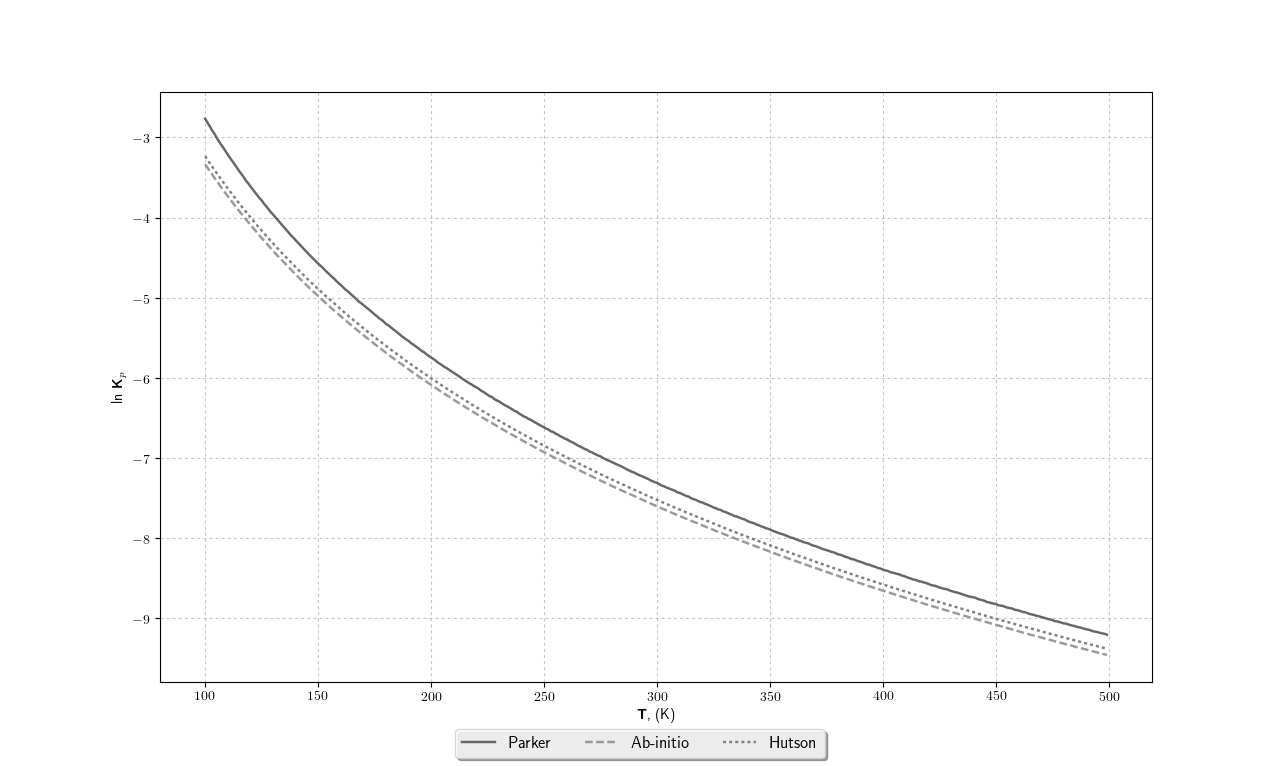
\includegraphics[width=1.1\textwidth]{pictures/all_eq_const.png}
	\caption{Зависимость логарифма константы равновесия от температуры}
	\label{fig:pic3}
\end{figure}

Следующим шагом стал расчет константы равновесия по выражению
\vverh
\begin{gather}
	K_p = \frac{4 \pi^2 N_A}{RT} \frac{ \lb Q_{bound}^{pair} \rb_{tr}}{Q_{Ar} Q_{CO_2}} \int\limits_{\mH < 0} \exp \lb - \frac{\mH}{k T} \rb d R \, d \theta \, d p_R \, d p_\theta \, d J_x \, d J_y \, d J_z \label{eqconstdim} 
\end{gather}

Расчет константы по выражению \eqref{eqconstdim} требует значительно большего компьютерного ресурса, однако позволяет рассчитывать константы равновесия для более сложных систем, для которых невозможно использовать техники, существенно уменьшающие размерность интеграла. В рамках следующего этапа мы отказались от аналитической формы гамильтониана. Расчет производился по тому же выражению \eqref{eqconstdim}, но гамильтониан $\mH$ в подынтегральном рассчитывался через матрицы лагранжиана $\bba, \bbA, \bbI$.



\newpage
\bibliographystyle{unsrt}
\bibliography{biblio}
\newpage

% modifying font of the appendix title
\appendix
\titleformat{\chapter}[display]
  {\normalfont\large\bfseries}% <- font for label "Appendix A", default \huge
  {\chaptertitlename\ \thechapter}{20pt}
  {\large}

  \section{Интегрирование экспоненциальной функции по объему многомерного шара \cite{huber1982}}
 \label{appendix:multint}
\begin{gather}
\left\{
\begin{aligned}
\vec{\Omega} = \frac{\partial \mathcal{H}}{\partial \vec{J}} \\ 
\vec{J} = \frac{\partial \mathcal{L}}{\partial \vec{\Omega}}
\end{aligned}
\right. \notag
\end{gather}

Доказательство первого соотношения представляет собой чисто техническую процедуру, так что опустим его. Продемонстрируем один из возможных путей доказательства второго соотношения:
\vverh
\begin{gather}
\vec{J} = \frac{\partial \mathcal{L}}{\partial \vec{\Omega}} = \bbA \dot{\vec{q}} + \bbI \, \vec{\Omega} \notag
\end{gather}

Для этого рассмотрим вектора углового момента в лабораторной системе координат и, используя ортогональную матрицу $\bbS$, выразим его через $\vec{\Omega}$ и $\left\{ \vec{R}_i \right\}$, представленные в подвижной системе координат:
\vverh
\begin{gather}
\vec{j} = \sum_{i=1}^{n} m_i \left[ \vec{r}_i \times \dot{\vec{r}}_i \right] \notag \\
\dot{\vec{r}}_i = \bbS^{-1} \lb \left[ \vec{\Omega} \times \vec{•}vec{R}_i \right] + \dot{\vec{R}}_i \rb \notag \\
\vec{j} = \sum_{i=1}^{n} m_i \left[ \vec{r}_i \times \bbS^{-1} \lb \left[ \vec{\Omega} \times \vec{R}_i \right] + \dot{\vec{R}}_i \rb \right] =
\bbS^{-1} \sum_i m_i \left[ \vec{R}_i \times \dot{\vec{R}}_i \right] + \bbS^{-1} \sum_i m_i \left[ \vec{R}_i \times \left[ \vec{\Omega} \times \vec{R}_i \right] \right] = \notag \\
= \bbS^{-1} \sum_i m_i \left[ \vec{R}_i \times \dot{\vec{R}}_i \right] + \bbS^{-1} \sum_i \lb R_i^2 \vec{\Omega} - \lb \vec{R}_i , \vec{\Omega} \rb \vec{R}_i \rb = \bbS^{-1} \bbA \dot{\vec{q}} + \bbI \, \vec{\Omega} \notag
\end{gather}

Умножая обе части на $\bbS$, приходим к искомому соотношению: 
\begin{gather}
\vec{J} = \bbS \vec{j} = \bbA \dot{\vec{q}} + \bbI \, \vec{\Omega} \notag 
\end{gather}

\section{Адаптивное интегрирование методом Монте-Карло \cite{lepage1978}}
\label{appendix:montecarlo}
Рассмотрим интеграл некоторой функции $n$ переменных $\mf{x} = \lb x_1, \dots, x_n \rb$ по некоторой области $\Omega \subset \mathbb{R}^n$:
\vverh
\begin{gather}
I = \int\limits_{\Omega} f \lb \mf{x} \rb d \mf{x} \label{mint1} 
\end{gather}

Будем оценивать интеграл \eqref{mint1} задавая некоторое случайное распределение $M$ точек по $\Omega$ с плотностью вероятности $\rho(\mf{x})$:
\vverh
\begin{gather}
S^{\lb 1 \rb} = \frac{1}{M} \sum_{\mf{x}} \frac{f \lb \mf{x} \rb}{\rho \lb \mf{x} \rb} \, \longrightarrow I, \text{при} \, M \longrightarrow \infty. \notag
\end{gather}

Построенная оценка интеграла $S^{\lb 1 \rb}$ также является случайной величиной, ей дисперсия равна:
\vverh
\begin{gather}
\sigma^2 = \frac{1}{M} \left[ \int\limits_{\Omega} \frac{f^2 \lb \mf{x} \rb}{\rho \lb \mf{x} \rb} d \mf{x} - \lb \int\limits_{\Omega} f \lb \mf{x} \rb d \mf{x} \rb^2 \, \right] \notag
\end{gather}

При больших $M$ дисперсия аппроксимируется следующим выражением:
\vverh
\begin{gather}
\sigma^2 \simeq \frac{1}{M - 1} \lb S^{\lb 2 \rb} - \lb S^{\lb 1 \rb} \rb^2 \rb, \quad S^{\lb 2 \rb} = \frac{1}{M} \sum_{\mf{x}} \lb \frac{f \lb \mf{x} \rb}{\rho \lb \mf{x} \rb} \rb^2. \notag
\end{gather}

Среднеквадратичное отклонение $\sigma$ показывает насколько точно величина $S^{\lb 1 \rb}$ оценивает интеграл $I$ \eqref{mint1}. Существует несколько техник уменьшения СКО $\sigma$ при фиксированном $M$:
\begin{itemize}
\item Выборка по значимости (\textit{Importance sampling}). Идея метода заключается в том, что некоторые значения случайной величины имеют б\'{o}льшую значимость (вероятность) для оцениваемой функции чем другие. Если более значимые значения будут вносить больший вес в оценку интеграла, то дисперсия уменьшится. Несложно убедиться, что оптимальное распределение $\rho \lb \mf{x} \rb$  есть
\vverh
\begin{gather}
\rho \lb \mf{x} \rb = \ddfrac{| f(\mf{x}) |}{\int\limits_{\Omega} |f(\mf{x})| d \mf{x}} \notag
\end{gather} 
То есть, идея метода заключается в "концентрировании" плотности $\rho \lb \mf{x} \rb$ в тех областях $\Omega$, где $| f \lb \mf{x} \rb |$ максимально. 
\item Стратифицированная выборка (\textit{Stratified sampling}). Идея этого метода заключается в разбиении объема $\Omega$ на $N$ более маленьких объемов разных размеров. Интегрирование методом Монте-Карло выполняется в каждом из маленьких объемов с использованием $\frac{M}{N}$ точек. Изменяя относительный размер и расположение маленьких объемов, мы изменяем их вклад как в значение интеграла, так и в дисперсию. Общее значение дисперсии становится минимальным, когда вклад каждого объема одинаков и равен $\frac{\sigma^2}{N}$.  
\end{itemize} 

В чистом виде эти методики не применимы для general purpose алгоритмов интегрирования (т.е. для таких алгоритмов, которые не используют априорного знания о поведении подынтегральной функции), однако разработаны итеративные алгоритмы, позволяющие использовать информацию о подынтегральной функции, полученной в ходе одной итерации, для улучшения оценки в следующей. \cite{lepage1978, tsuda1973, haselgrove1961}


\end{document}
